\documentclass{article}

% Package imports
\usepackage{titlesec}
\usepackage{geometry}
\usepackage{fancyhdr}
\usepackage{graphicx}
\usepackage{hyperref} % \url, https://www.overleaf.com/learn/latex/Hyperlinks
\usepackage{outlines} % better itemize
\usepackage{comment}
\usepackage{multirow} % tables
\usepackage{noto} % Google Noto Fonts

\usepackage[british]{datetime2} % load before gitinfo2 to customize
\usepackage[mark=true,grumpy=true]{gitinfo2}

% Redefine \gitMark to customize it
% https://mirror.apps.cam.ac.uk/pub/tex-archive/macros/latex/contrib/gitinfo2/gitinfo2.pdf
\renewcommand{\gitMark}{Branch: \gitBranch\,@\,\gitAbbrevHash{}\,\textbullet{}\,\DTMusedate{gitdate}}

\geometry{a4paper, includeheadfoot, portrait, total={}, top=12.5mm, bottom=12.5mm, left=25.4mm, right=25.4mm}

\graphicspath{ {./images/} }

% Variables
\def\projectname{Inventory Project}

% Override subparagraph with a variant that has no indentation
% https://tex.stackexchange.com/a/392014
\makeatletter
\renewcommand\subparagraph{%
\@startsection{subparagraph}{5}{0pt}%
{3.25ex \@plus 1ex \@minus .2ex}{-1em}%
{\normalfont\normalsize\bfseries}}
\makeatother

\title{\projectname}
\author{James Cahill}
\date{Sepetember 2023}

% Configure fancyHDR page style
% https://tex.stackexchange.com/questions/266911/get-fancyhdr-and-geometry-to-work-nicely
\fancypagestyle{style}{
    \fancyhead{} % clear all header fields
    \fancyhead[HL]{\projectname}
    \fancyhead[HR]{James Cahill}
    \renewcommand{\headrulewidth}{0pt} % Remove header line
}
\pagestyle{style}


\begin{document}


\tableofcontents

\pagebreak

\section{Analysis}

% Background
\subsection{Problem Identification}

\subsubsection{Problem Description}

Popular inventory management solutions are relatively expensive, and may be out
of reach for individuals or small schools.
Inventory systems have numerous benefits for businesses and individuals alike; a business
may choose to track their supply levels where an individual may wish to catalogue their DVD collection. \\

\noindent My goal is to create a web-based application aimed at both businesses and individuals to manage
inventory, with additional modern features such as automatic item re-ordering when stocks are running low.\\

\noindent Traditional inventory management solutions are typically single-user at best, whereas I intend to create
a multi-user, collaborative environment.\\

\noindent In my view, an inventory system should be:

\begin{outline}
    \1 Easy for end users to use.
    \1 Cross platform
    \1 Performant interface
    \1 Efficient in terms of adding data
    \1 Allow for easy cataloguing of inventory
    \1 Allow for item scanning using QR codes / barcodes
    \1 Be able to source data from external sources
    \1 Support both consumable and non-consumable goods.

    
\end{outline}


\begin{comment}
An inventory system should be able to:

time consuming to add data
not user friendly

- catalogue of inventory, re-order for you
- scan using a phone (no external hardware needed)
- alert / re-order when stocks are running low.
- purchase links
- stretch: source data from amazon or equivalent instead of typing it manually
- search engine for catalogued and new Parts
    - provides with options for where to purchase certain goods
- button to re-order
    - smart device???????
- predict when stocks will run out.
- source data from external sources
- like monzo projection of when it will run out
- how much you are spending each month on goods
- nfc support to easily scan / etc items (might be too hard on iOS)
\textbf{Barcode check in / out}
- monzo integration
- budgeting - figure projections  as well 
clearly define what the APP will feature.
Think about
- potential users
    - how does the app cater to their needs - different features etc


\end{comment}

\subsubsection{Stakeholders}

\newcommand{\stakeholderEntry}[4]{{#1} & {#2} & {#3} & {#4}\\\hline}

\begin{tabular}{ |c|p{0.2\textwidth}|c|c| }
    \hline
    \textbf{Stakeholder} & \textbf{Description} & \textbf{Current Use} & \textbf{Requirements}\\
    \hline

    \stakeholderEntry
        {Claire Foley}
        {
            \begin{outline}
                \1 SENCo
                \1 Library Lead
            \end{outline}
        }
        {
            No system. Library books are not tracked.
        }
        {TBD}

    \hline
\end{tabular}


\subsubsection{Interview}

\pagebreak

\subsubsection{Existing similar solutions}

% do 4-5 alternatives

% 1. InvenTree
\paragraph{\\InvenTree}
\url{https://inventree.org/}

\subparagraph{\\Overview\\}

InvenTree is an \textbf{open-source} inventory management system, providing \textit{low level stock control and part tracking}.
It uses a Python/Django database backend and provides both a \textbf{web-based interface} as well as a REST API for interacting with other services.
InvenTree also has a powerful plugin system for custom applications and other extensions. \\

\noindent Below is a screenshot of the InvenTree homepage.\\
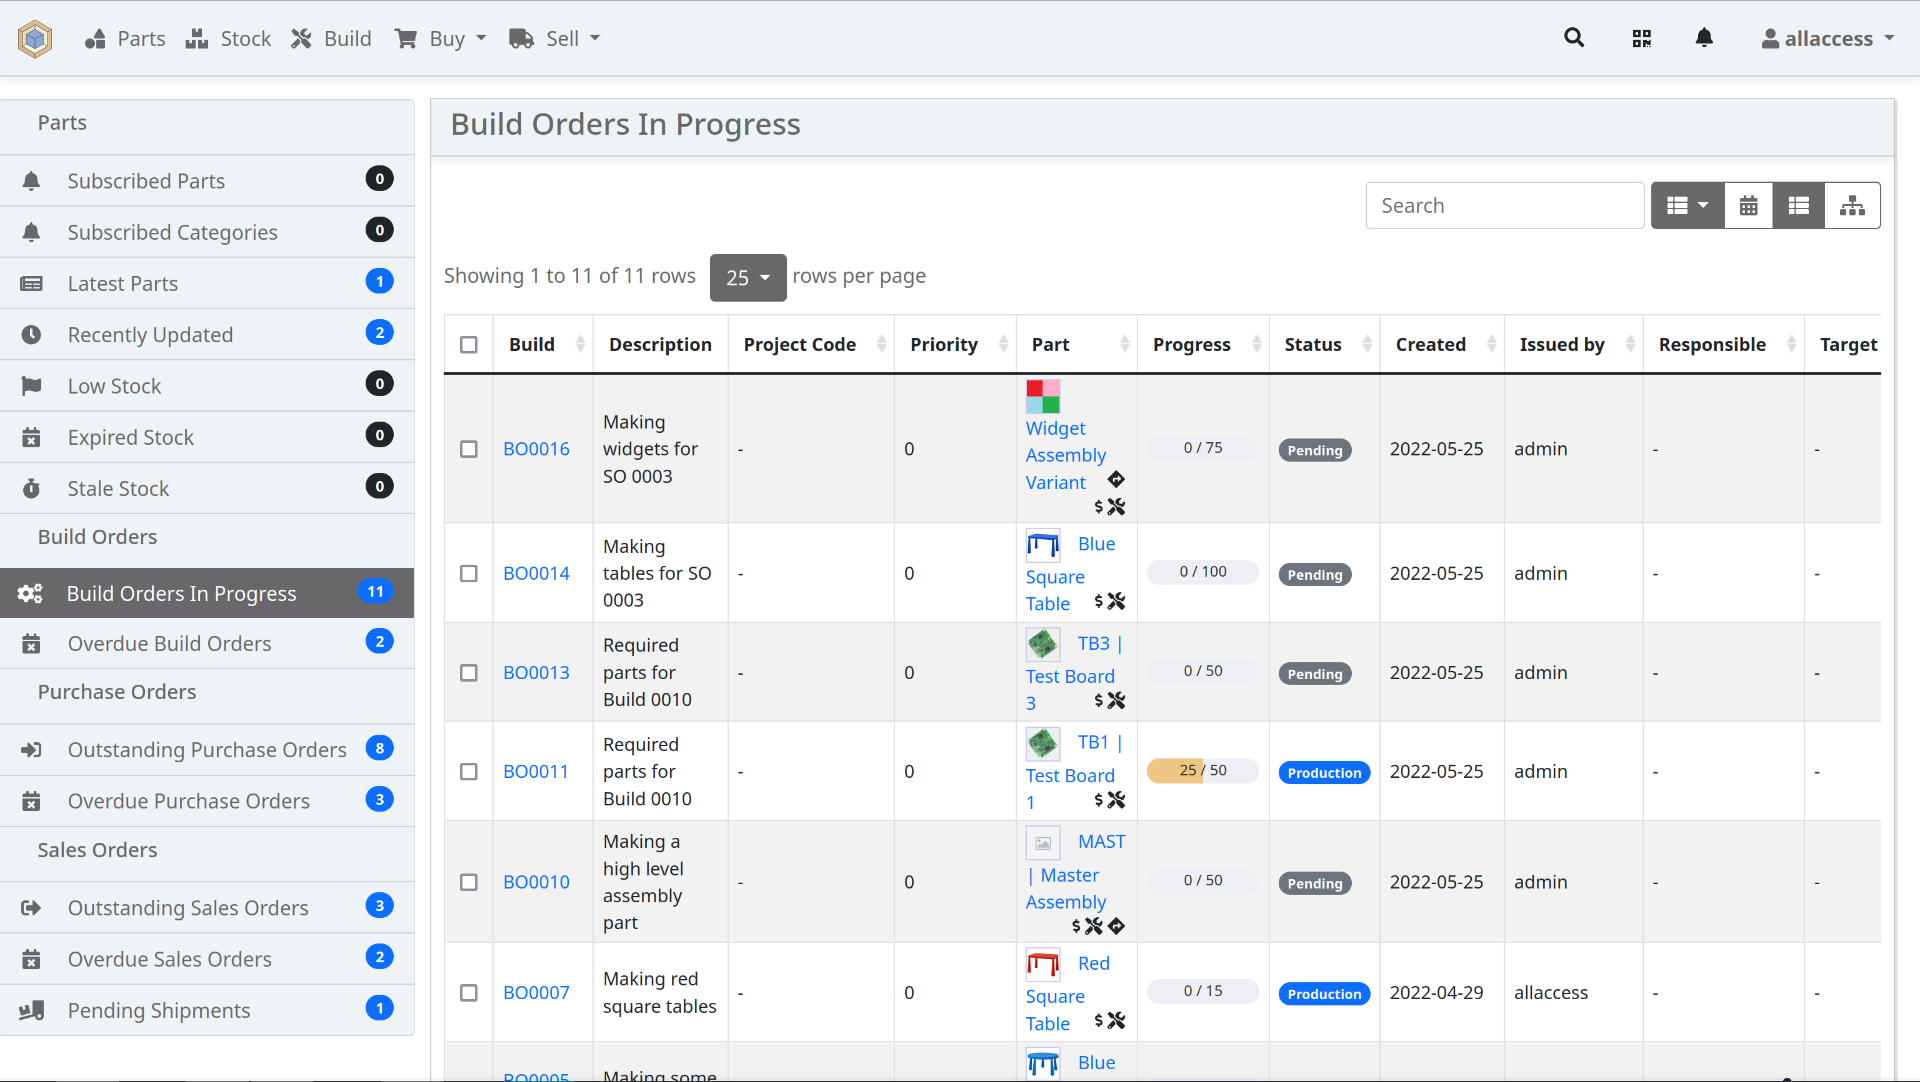
\includegraphics[width=15cm]{inventree_demo_homepage.png}

\subparagraph{Parts applicable to my solution\\}

- concept is similar (web-based), but I'm doing a different approach.\\
\noindent - not indented for stock control

\pagebreak

% 2. PartKeepr
\paragraph{\\PartKeepr}
\url{https://partkeepr.org/}\\

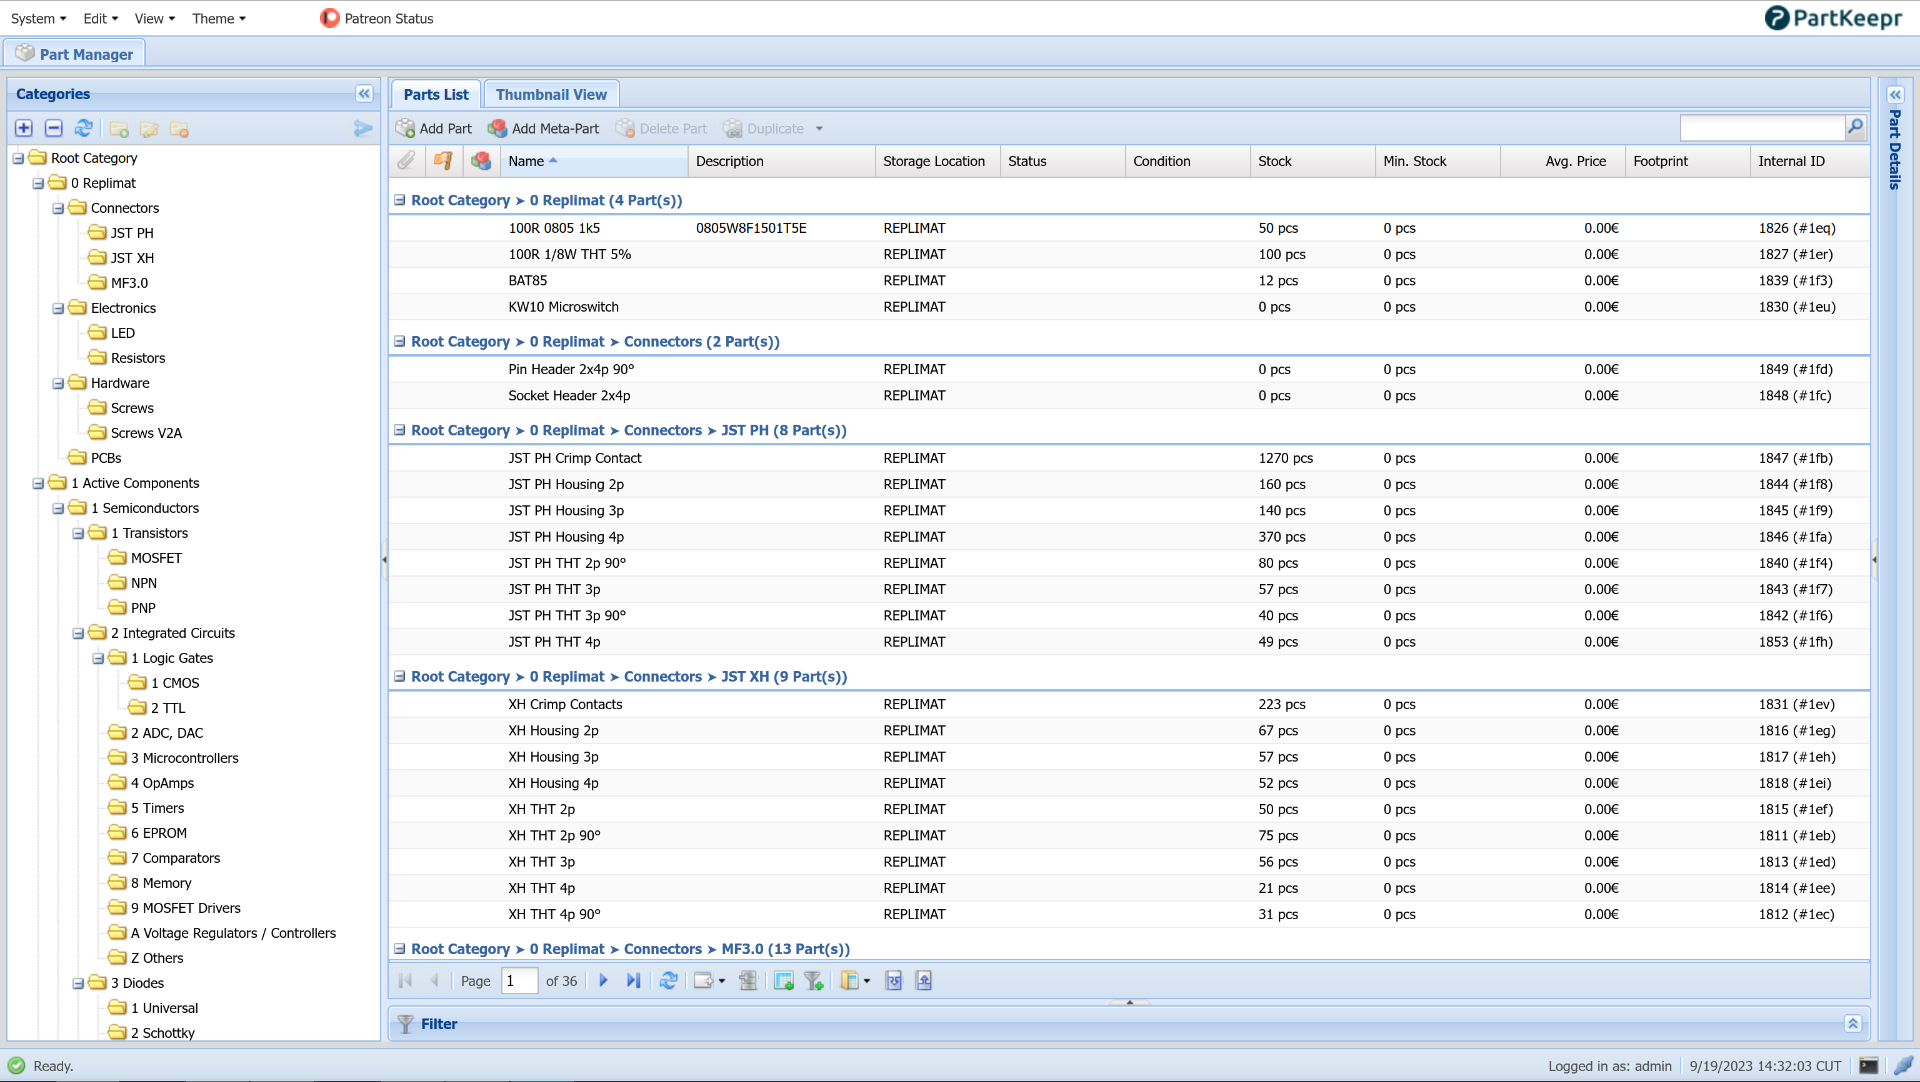
\includegraphics[width=15cm]{partkeepr_demo_homepage.png}

\subparagraph[indent=false]{\\Overview\\}

PartKeepr is an open-source inventory management system with a focus on electronic components.
It is designed around four main principles:

\begin{outline}
    \1 Fast Part Searching
    \1 Ability to add complete part database
    \1 Keeping track of stock
    \1 Ease of use
\end{outline}

\subparagraph{Parts applicable to my solution\\\\}

\noindent Like PartKeepr, I hope to implement a web-based interface.
However, I am using a different approach as my solution will not be tailored specifically to electronic components.

\pagebreak

% 3. Sortly
\paragraph{\\Sortly}
\url{https://www.sortly.com/solutions/inventory-management-software/}\\

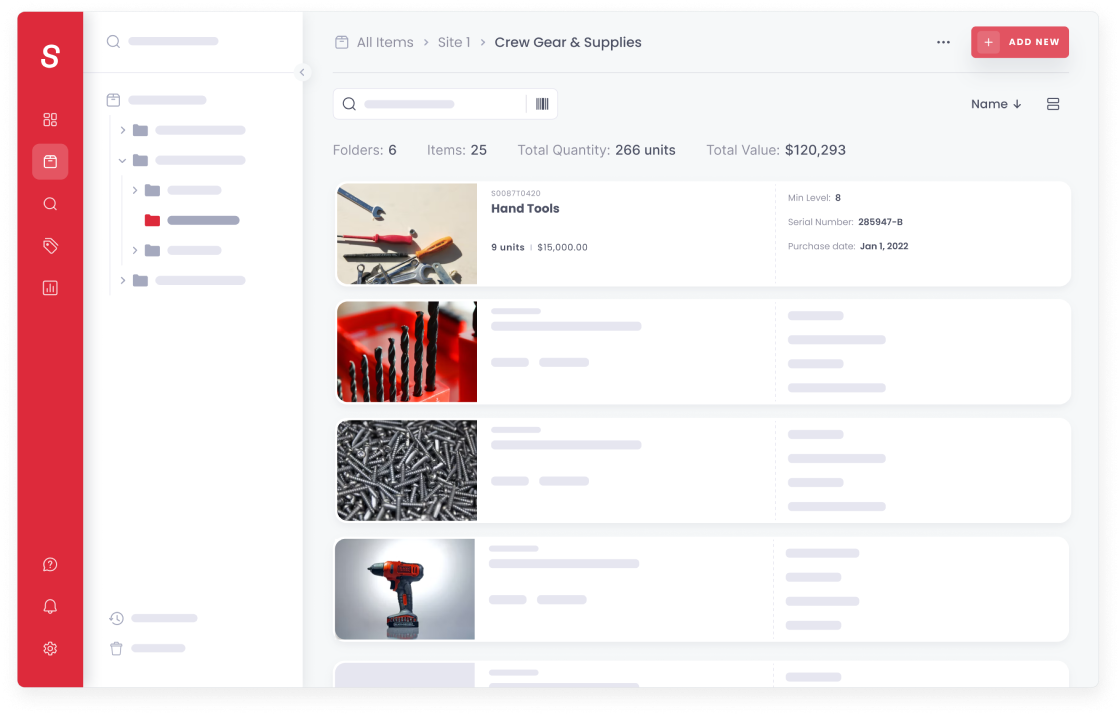
\includegraphics[width=15cm]{sortly_homepage_mockup_1.png}

\subparagraph{\\Overview\\}

Sortly is a proprietary cloud-based inventory management system with a focus on small businesses and inviduals.\\\\
It has two plans available, an always free plan with limited functionality and a paid plan will a more complete feature-set.

\subparagraph{Parts applicable to my solution\\\\}

I hope to implement the following features from Sortly:

\begin{outline}
    \1 Web based interface
    \2 Allows for easy access.

    \1 Barcode support
    \2 Allows end users to print off QR codes to stick to items
    \2 Which can be scanned in-app to easily perform actions on the item.

    \1 Real-time reporting insights
    %\subitem 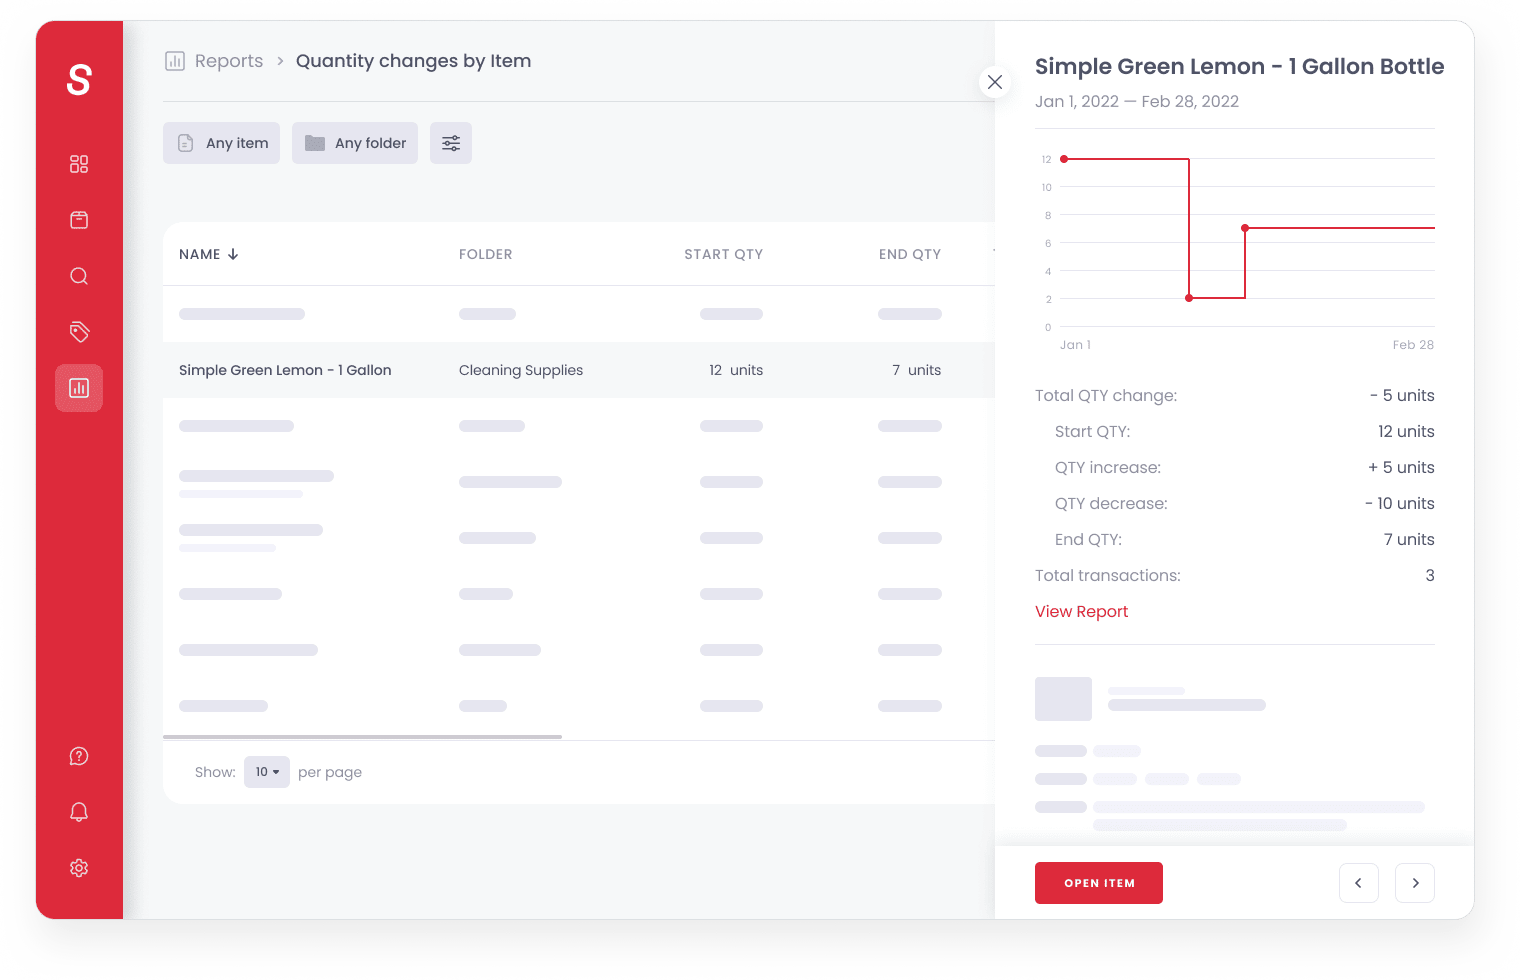
\includegraphics[width=10cm]{sortly_homepage_mockup_2.png}
    \2 Allows for added insight into usage patterns for particular units.
\end{outline}

\subsubsection{Features to be incorporated into solution}

\subsubsection{Feedback from stakeholders}

\subsection{Requirements}

\subsubsection{Stakeholder requirements}

\subsubsection{Software and hardware requirements}

\subsubsection{Success requirements}

\section{Design}

\subsection{User Interface Design}

\subsubsection{Usability Features}

\subsubsection{Feedback from stakeholder}

\subsection{Modular breakdown}

\subsection{Algorithms}

\subsection{Data Dictionary}

\subsection{Inputs and outputs}

\subsection{Validation}

\subsection{Testing}

\subsubsection{Methods}

\subsubsection{Test Plan}

\section{Implementation}

\subsection{First Iteration}

\section{Testing}

\section{Evaluation}

\end{document}